\section{Klasse diagrammer}

\subsection{Webapplikation}

\subsubsection{FlightPathHandling}
På klasse diagrammet FlightPathHandling ses de tre overordnet klasser hvilket udgør pakken FlightPathHandling pakken som vist på figur \ref{fig:pakke_diagram}.

\vspace{-5pt}
%kommentar
\begin{figure}[H]
	\centering
	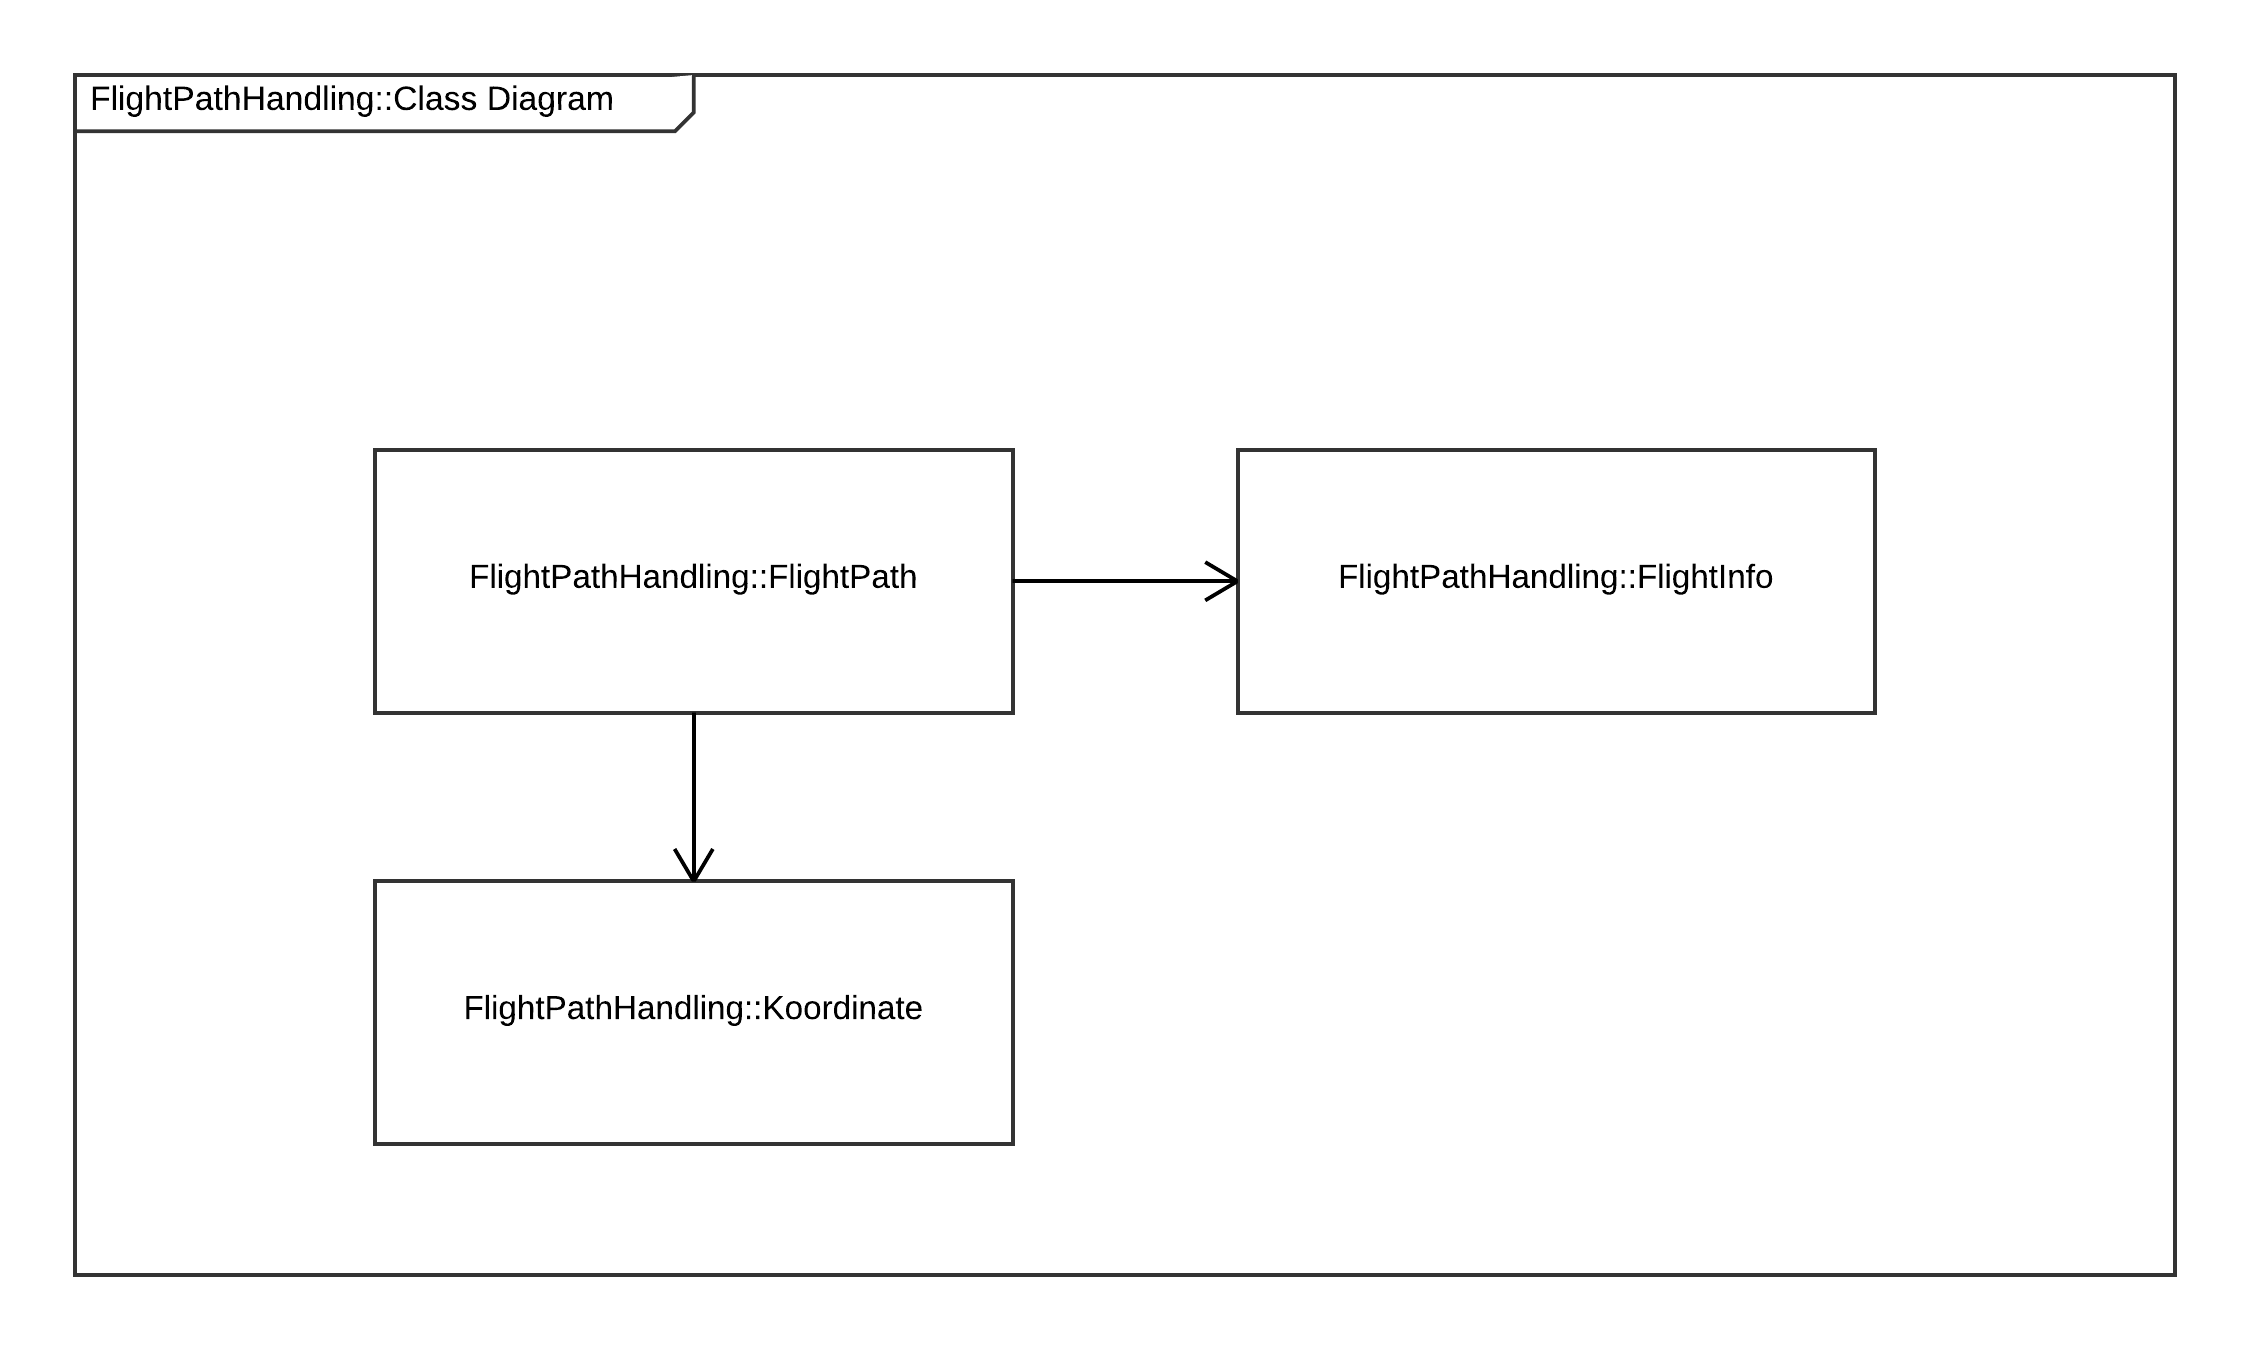
\includegraphics[width=0.7\textwidth]{Billeder/klasse_diagrammer/FlightPathHandlingDiagram.png}
	\vspace{-5pt}
	\caption{FlightPathHandling klasse diagram}
	\label{fig:FlightPathHandling_klasse_diagram}
\end{figure}

\textbf{FlightPath}\\
Klassen FlightPath bruger både FlightInfo og Coordinate klasserne til at udgøre en FlightPath.

\textbf{Coordinate}\\
Coordinate klassen håndtere det GPS koordinater som brugeren ønsker dronen skal flyve til.

\textbf{FlightInfo}\\
FlightInfo klassen håndtere data om ruten så som flyvehøjde, dato for flyvning.

\textbf{FileHandling}\\
FileHandling klassen genere en fil ud fra data'en i FlightPath som så sendes til dronen.

\textbf{JSONFormat}\\
Klassen nedarver fra FileHandling for at kunne bruges som FileHandling. Klassen genere en JSON fil som kan sendes til dronen.

\newpage
\subsubsection{UserHandling}
Klasse diagrammet viser hvilket klasser som udgør UserHandling pakken som vist på figur \ref{fig:pakke_diagram}.

\vspace{-5pt}
%kommentar
\begin{figure}[H]
	\centering
	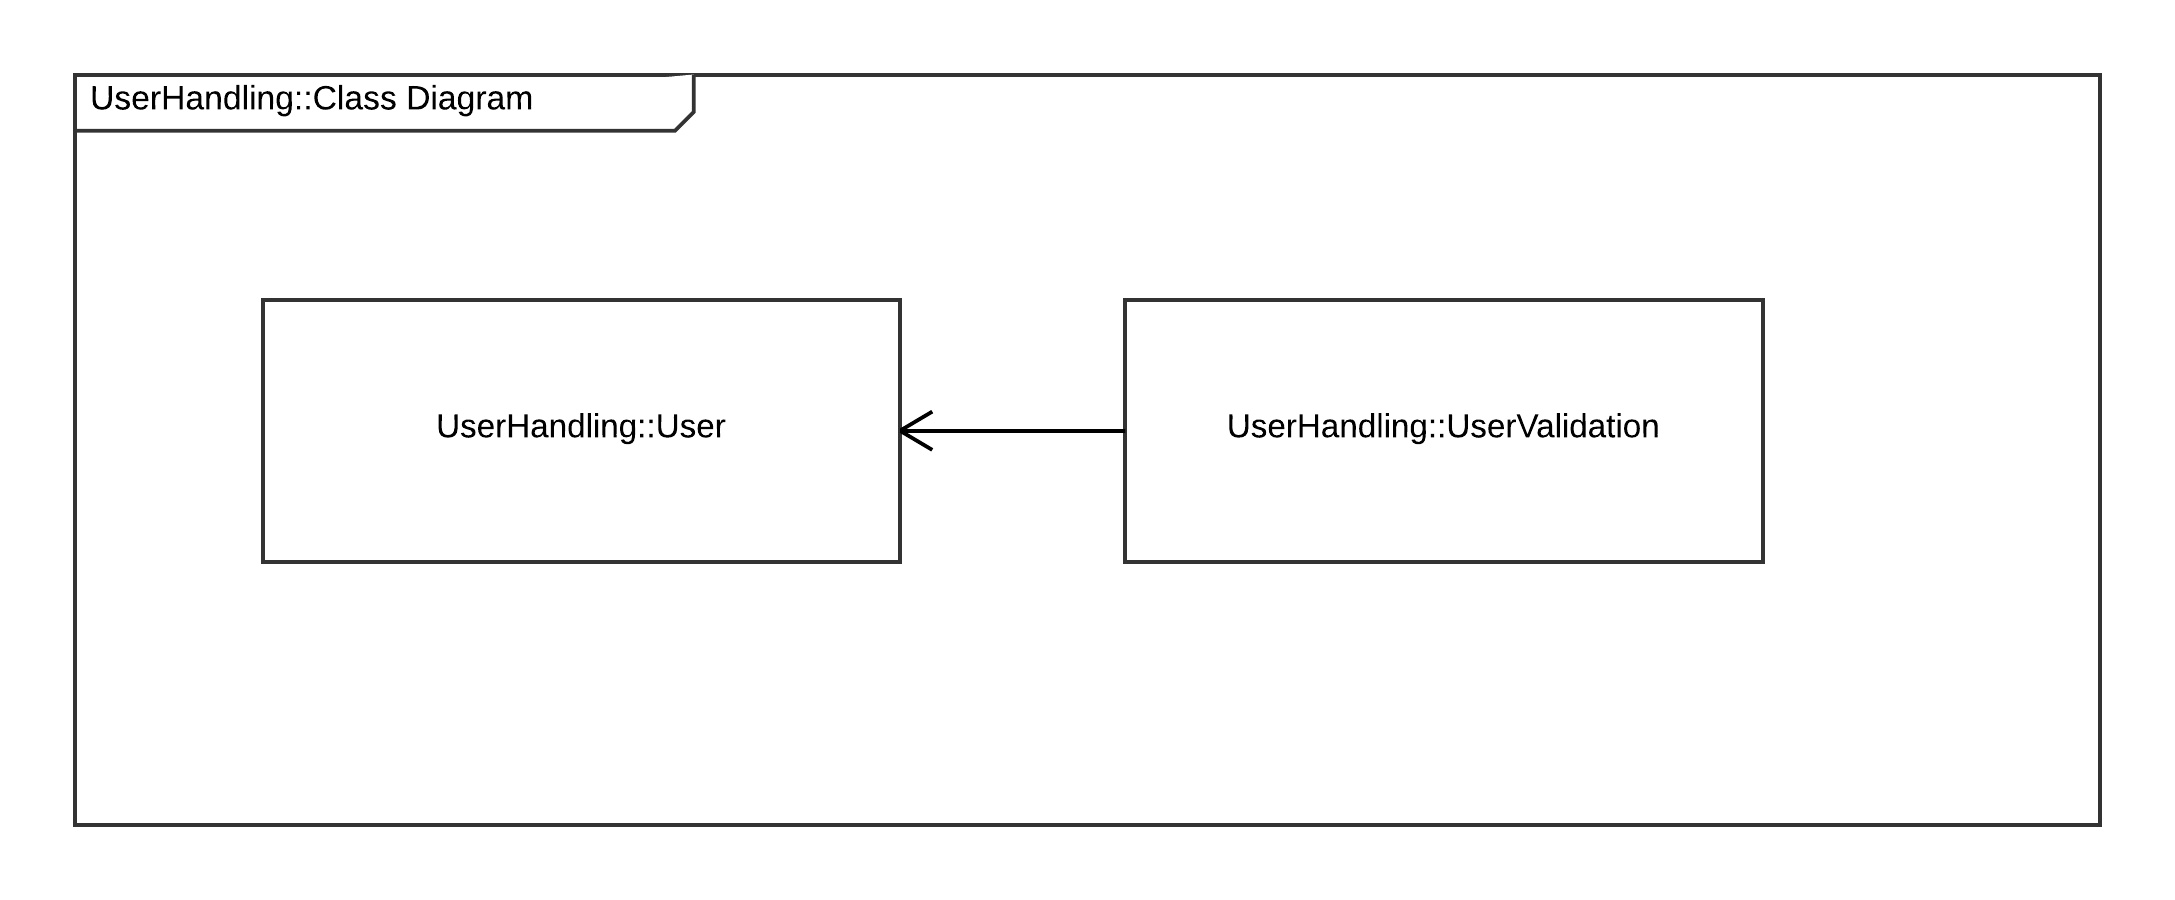
\includegraphics[width=0.7\textwidth]{Billeder/klasse_diagrammer/UserHandlingDiagram.png}
	\vspace{-5pt}
	\caption{UserHandling klasse diagram}
	\label{fig:UserHandling_klasse_diagram}
\end{figure}

\textbf{User}\\
User klassen indeholder alle data om brugerne i systemet. Klassen bliver også brugt af UserValidation i forbindelse med login/log out.

\textbf{UserValidation}\\
UserValidation klassen har ansvaret for at validere en user når der bliver forsøgt login.\\

\newpage
\subsubsection{DatabaseHandling}
Klasse diagrammet viser hvilket klasser som udgør DatabaseHandling pakken som vist på figur \ref{fig:pakke_diagram}.

\vspace{-5pt}
%kommentar
\begin{figure}[H]
	\centering
	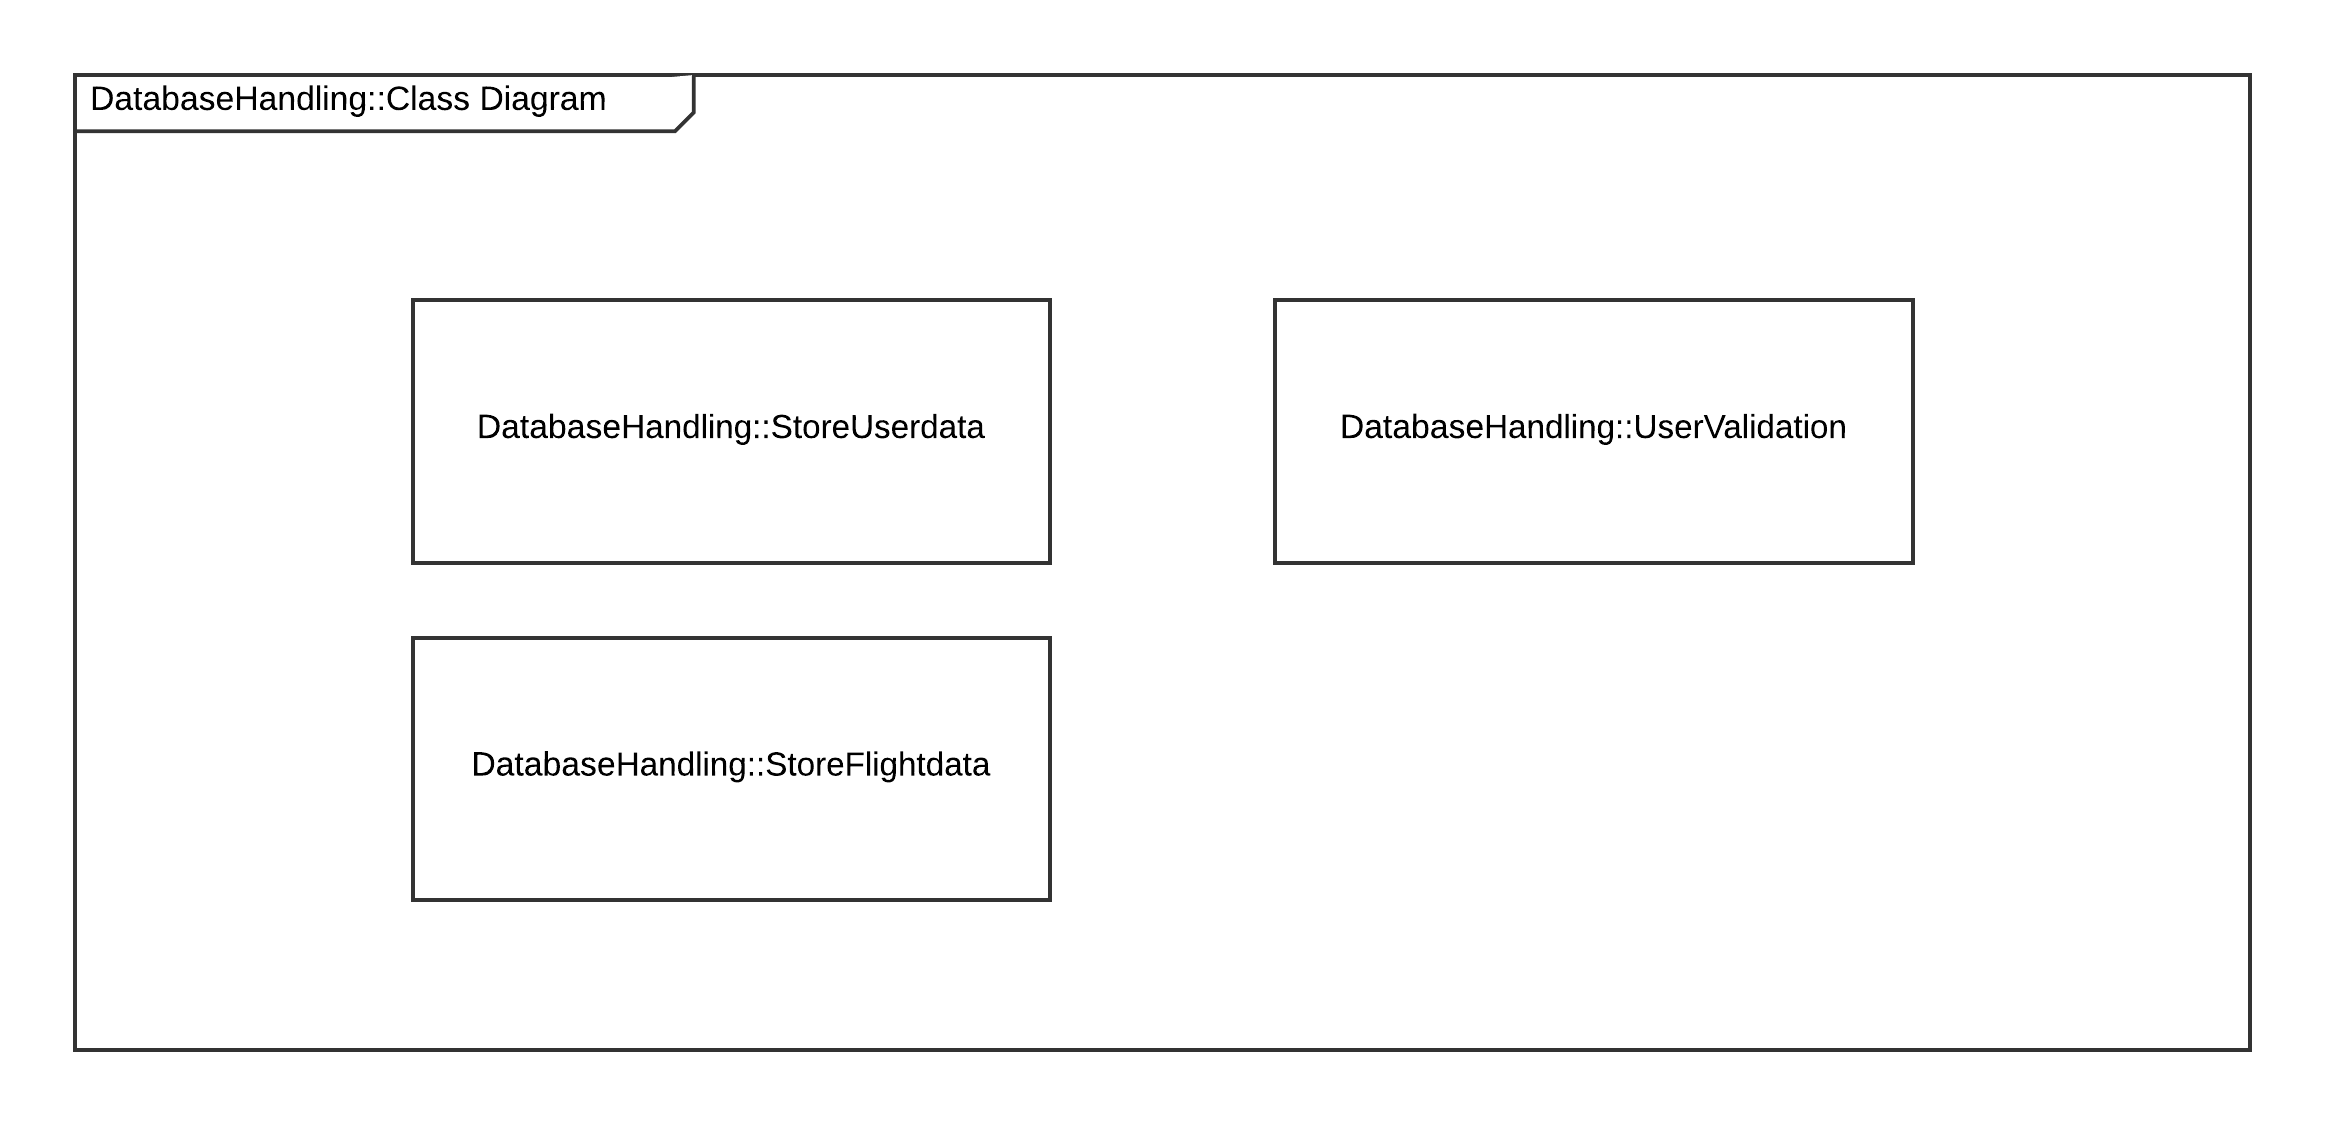
\includegraphics[width=0.7\textwidth]{Billeder/klasse_diagrammer/DatabaseHandling.png}
	\vspace{-5pt}
	\caption{DatabaseHandling klasse diagram}
	\label{fig:DatabaseHandling_klasse_diagram}
\end{figure}

\textbf{DatabaseConnection}\\
Superklassen DatabaseConnection har til ansvar at skabe forbindelse til databasen og lukke kommunikationen ned efter data overførelse. De andre klasser nedarver fra klassen så de kan oprette forbindelse og lukke forbindelsen.

\textbf{StoreUserdata}\\
Klassen opdatere brugerdata i databasen. Igennem nedarvningen fra superklassen DatabaseConnection kan StoreUserdata også oprette forbindelse og lukke forbindelsen igen til databasen.

\textbf{StoreFlightdata}\\
StoreFlightdata gemmer alle data omkring flyvning. Denne klasse bruges løbende under flyvning når billeder bliver modtaget og skal gemmes til en igangværende flyvning.

\textbf{UserValidation}\\
UserValidation validaere bruger ved forsøg på login og giver adgang til systemet hvis brugeren er valid.

\newpage
\subsubsection{CommunicationHandling}
Klasse diagrammet viser hvilket klasser som udgør CommunicationHandling pakken som vist på figur \ref{fig:pakke_diagram}.

\vspace{-5pt}
%kommentar
\begin{figure}[H]
	\centering
	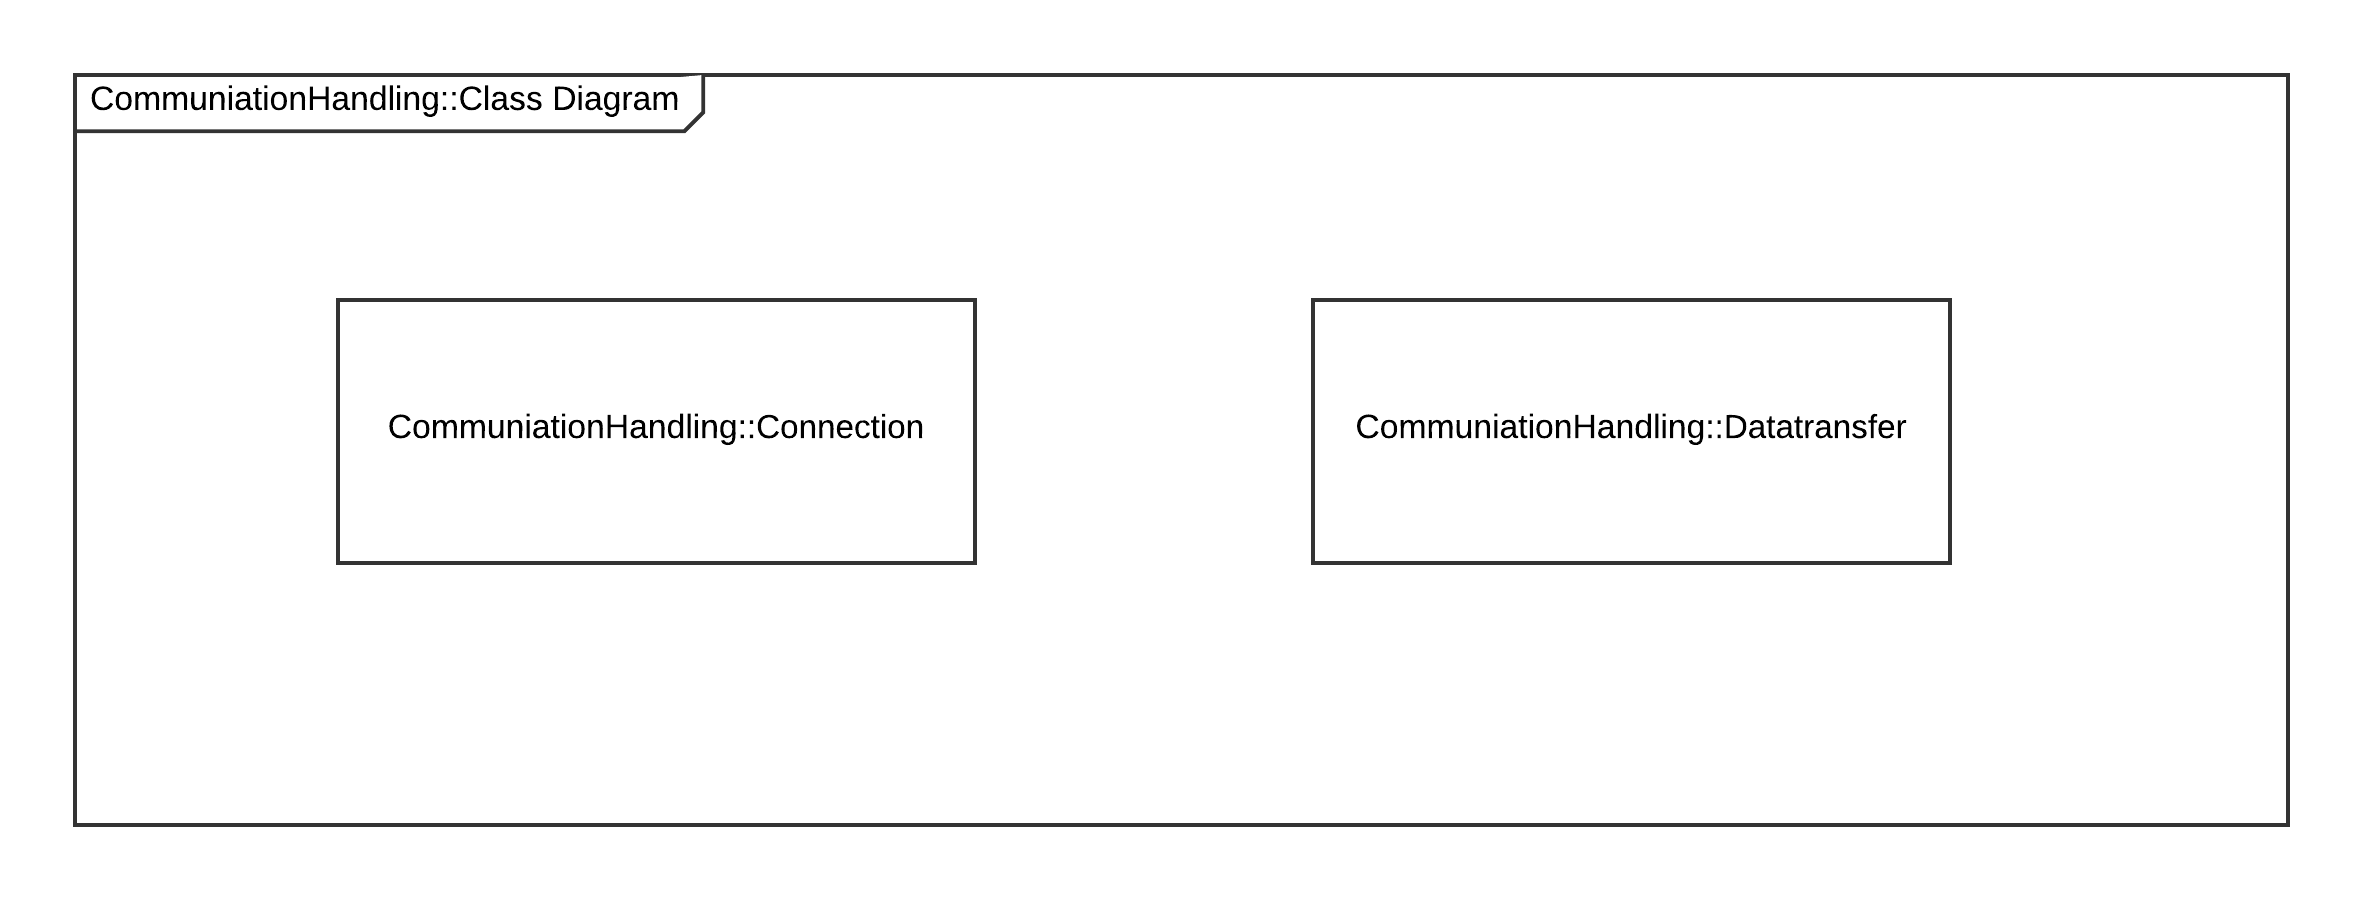
\includegraphics[width=0.7\textwidth]{Billeder/klasse_diagrammer/CommunicationHandling.png}
	\vspace{-5pt}
	\caption{CommunicationHandling klasse diagram}
	\label{fig:CommunicationHandling_klasse_diagram}
\end{figure}

\textbf{Connection}\\
Connection klassen har til ansvar for at skabe forbindelse imellem serveren og dronen.

\textbf{Datatransfer}\\
Datatransfer klassen bruger connection klassen til at oprette forbindelse til dronen inden data'en sendes. 
